\documentclass{article}
\usepackage[utf8]{inputenc}
\usepackage{graphicx}
\graphicspath{ {./pics/} }
\usepackage{placeins}
\usepackage{dirtytalk}
\usepackage{fancyhdr}
\usepackage{alltt}
\usepackage[document]{ragged2e}
\usepackage{wrapfig}

\setlength{\headheight}{15.2pt}
\pagestyle{fancy}
\fancyhf{}
\fancyhead[L]{2019-05-14}
\fancyhead[C]{TDP019 Projekt: Datorspråk}
\fancyhead[R]{Eric Jönsson \\ Vidar Siwe}
\fancyfoot[C]{\thepage}

\title{TDP019 Projekt: Datorspråk}
\author{Eric Jönsson och Vidar Siwe}
\date{2019-05-14}

\begin{document}

%----------------------------------------------------------------------------------------
%	TITLE PAGE
%----------------------------------------------------------------------------------------

\begin{titlepage} % Suppresses displaying the page number on the title page and the subsequent page counts as page 1
	\newcommand{\HRule}{\rule{\linewidth}{0.5mm}} % Defines a new command for horizontal lines, change thickness here
	
	\center % Centre everything on the page
	
	%------------------------------------------------
	%	Headings
	%------------------------------------------------
	
	\textsc{\LARGE Linköpings universitet}\\[1.5cm] % Main heading such as the name of your university/college
	
	\textsc{\Large TDP019}\\[0.5cm] % Major heading such as course name
	
	\textsc{\large Projekt: Datorspråk}\\[0.5cm] % Minor heading such as course title
	
	%------------------------------------------------
	%	Title
	%------------------------------------------------
	
	\HRule\\[0.4cm]
	
	{\huge\bfseries CodEng}\\[0.4cm] % Title of your document
	
	\HRule\\[1.5cm]
	
	%------------------------------------------------
	%	Author(s)
	%------------------------------------------------
	
	\begin{minipage}{0.4\textwidth}
		\begin{flushleft}
			\large
			\textit{Author}\\
			Eric \textsc{Jönsson}\\
			Vidar \textsc{Siwe} % Your name
		\end{flushleft}
	\end{minipage}
	~
	\begin{minipage}{0.4\textwidth}
		\begin{flushright}
			\large
			\textit{Examinator}\\
			Jonas \textsc{Wallgren} % Supervisor's name
		\end{flushright}
	\end{minipage}
	
	% If you don't want a supervisor, uncomment the two lines below and comment the code above
	%{\large\textit{Author}}\\
	%John \textsc{Smith} % Your name
	
	%------------------------------------------------
	%	Date
	%------------------------------------------------
	
	\vfill\vfill\vfill % Position the date 3/4 down the remaining page
	
	{\large\today} % Date, change the \today to a set date if you want to be precise
	
	%------------------------------------------------
	%	Logo
	%------------------------------------------------
	
	\vfill\vfill
	\includegraphics[width=0.2\textwidth]{lith.png}\\[1cm] % Include a department/university logo - this will require the graphicx package
	 
	%----------------------------------------------------------------------------------------
	
	\vfill % Push the date up 1/4 of the remaining page
	
\end{titlepage}

\newpage
\tableofcontents
\newpage

\section{Inledning}
TDP019 Projekt: datorspråk är ett av de projektarbeten som görs av studenter som läser första året på programmet Innovativ programmering vid Linköpings universitet. Projektet utförs under hela den andra terminen och redovisas i maj. Projektet går ut på att ett eget programmeringsspråk ska konstrueras och implementeras. \\ \newline 
Det konstruerade språket programmeras i programmeringsspråket Ruby och till hjälp finns en redan programmerad parser kallad rdparse. Det programmeringsspråk som vi har skapat kallas för \say{CodEng}. Språket går ut på att i stor del kunna skrivas som \say{normal} text på engelska. 

\section{Användarhandledning}
\say{CodEng} som ord kommer ifrån en sammansättning av delarna \say{cod} från \say{code} och \say{eng} från \say{english}. Språket fick detta namn för att det ska vara intuitivt angående vad språkets grundidé är. Språket är ett imperativt programmeringsspåk och går ut på att det i stor utsträckning ska fungera att skriva ut programmeringskoden som engelsk text. För att kunna skriva språket som ren text behövs förkunskaper i programmering, eftersom de ord som är godkända att använda är baserade på hur \say{normal} programmering ser ut. Språket riktar sig mot de personer som vill att koden de skriver ser mer ut som normal text än kod i sina programmeringsfiler.

\subsection{Installation}
CodEng kräver linux med senaste versionen av programmeringsspråket Ruby. I skrivande stund är det version 2.6.3. Ladda ner \say{CodEng} till valfri plats och öppna sedan terminalen i undermappen \textbf{bin}. Skriv sedan följande kommando i terminalen för att slutföra installationen: \\ \newline
\texttt{\textbf{echo "PATH=\$PATH:\$(pwd)" >> <konfigurationsfil>}} \\ \newline
Ersätt \(<\)konfigurationsfil\(>\) med sökvägen till skalets konfigurationsfil. För bash är detta \texttt{\textbf{\textasciitilde/.bashrc}}. Starta om terminalen eller ladda konfigurationsfilen igen för att slutföra installationen.

\subsection{Körning}
CodEng kan köras på två sätt, interaktivt eller med en fil. Skriv följande kommando i terminalen för att köra en fil: \newline
\texttt{\textbf{CodEng <sökväg-till-fil>}} \newline
Ifall ingen fil anges körs CodEng i interaktivt läge. I interaktivt läge får användaren själv mata in kommandon på en rad som sedan parsern tolkar.
Ett returvärde skrivs sedan ut i terminalen och användaren får möjlighet att mata in igen.

\subsection{Datatyper}
Det finns fem stycken olika datatyper i CodEng. Datatyperna är CEBool, CEFloat, CEInteger, CEString och CEVariable. \\ \newline
CEBool är den datatyp i språket som hanterar \say{true}- och \say{false}-värden. Detta betyder att om ett sant eller falskt värde skapas i språket kommer det värdet att sparas som ett objekt av typen CEBool. Denna sortens sparning gäller generellt för alla de olika datatyperna men värdena som sparas i dem skiljer sig från varandra.
\\ \newline I CEFloat sparas decimaltal som skrivs i koden eller som beräknas av programmets körning.
CEInteger sparar på samma sätt som CEFloat tal. Skillnaden är att CEInteger endast sparar heltal. 
CEString är den datatyp som sparar textsträngar i språket till exempel sparas \say{3} som en CEString men 3 sparas som en CEInteger. Skillnaden för att det ska sparas som en textsträng är att det som ska sparas skrivs inom citattecken. I datatypen CEVariable sparas de variabler som sätt i koden.


\subsection{Operationer}
I språket hanteras tre stycken olika typer av operationer. Aritmetiska operationer, relationsoperationer och logiska operationer. \\ \newline
I de aritmetiska operationerna används operatorerna: +, -, *, /, ** och () för att strukturera upp de aritmetiska uttryck som kan tänkas utföras med språket. I språket motsvaras också operatorerna av engelska textversioner. Några exempel på aritmetiska uttryck och hur de kan skrivas i CodEng på olika sätt visas i figur 1.

\FloatBarrier
\begin{figure}[h!]
    \centering
    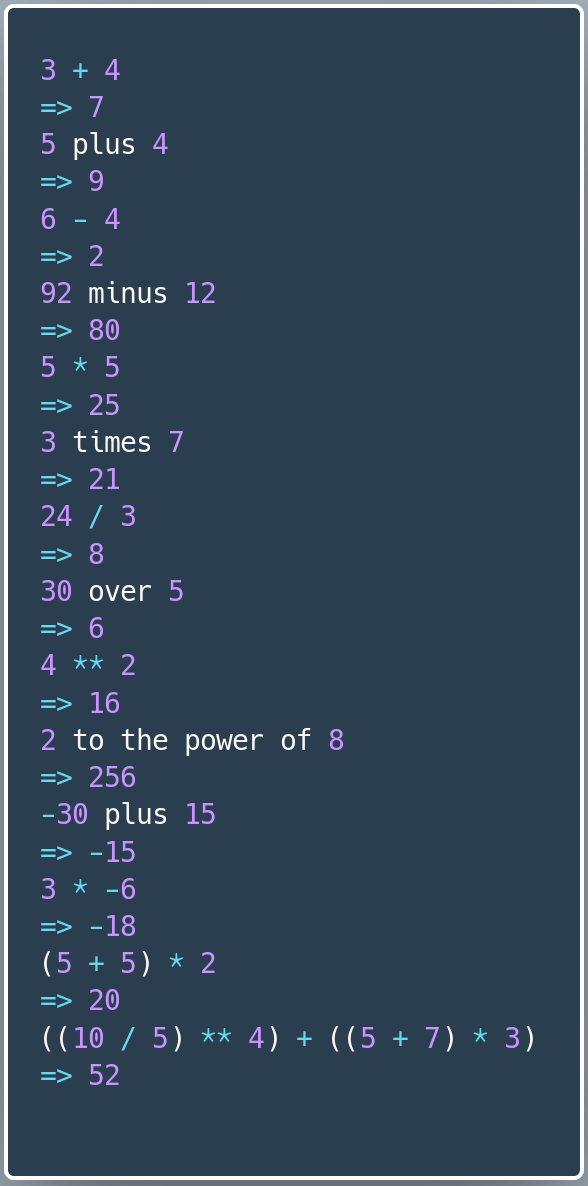
\includegraphics[width=0.35\textwidth]{arithm.png}
    \caption{Aritmetiska uttryck och hur de kan skrivas i CodEng.}
    \label{fig:arithm1}
\end{figure}
\FloatBarrier

Den andra typen av operationer som har implementerats i programmeringsspråket var relationsoperationer. Operatorerna för relationsoperationer är: \(<, <=, >, >=\), ==, != och de används för att hitta hur olika värden relaterar i förhållande till varandra. Exempelvis används de ofta inom iterationer för att se om loop är färdig eller inte. I CodEng finns det speciella uttryck som motsvarar dessa operatorer. Olika typer av relationsuttryck visas med exempel i figur 2.

\FloatBarrier
\begin{figure}[h!]
    \centering
    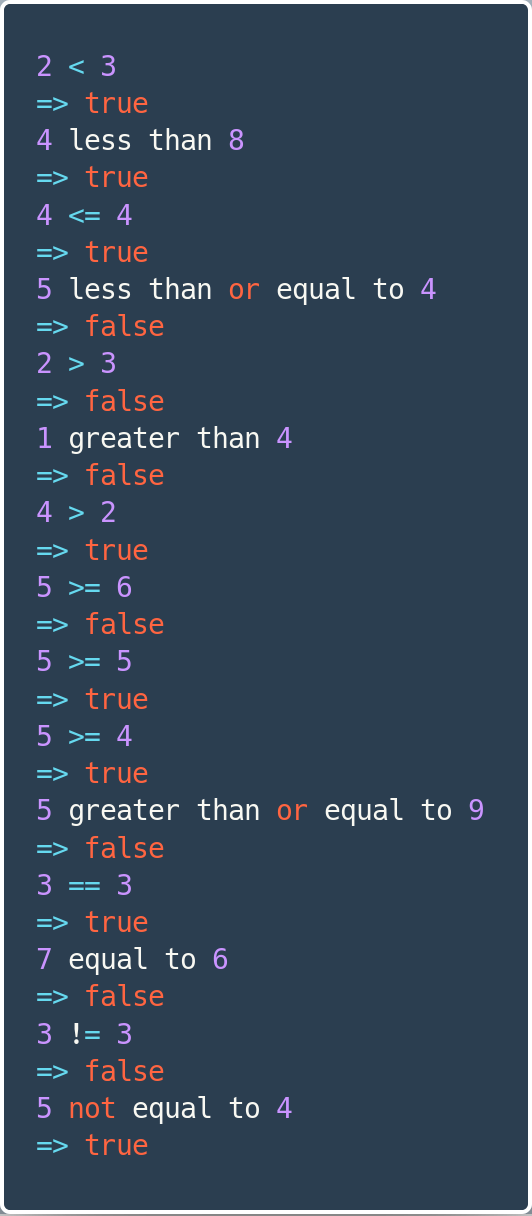
\includegraphics[width=0.35\textwidth]{relation.png}
    \caption{Relationsoperationer och hur de kan skrivas i CodEng.}
    \label{fig:rel1}
\end{figure}
\FloatBarrier

Logiska operatorer används i logiska uttryck för att se om värdet blir sant eller falskt. Operatorerna är:
\&\&, \(\mid \mid\) och ! som motsvaras av \say{and}, \say{or} och \say{not} i CodEng. Exempel på hur logiska uttryck kan användas i språket syns i figur 3. Vid användning av logiska operatorer på siffror räknas alla siffror som inte är 0 som sanna värden, endast 0 räknas som falskt.


\FloatBarrier
\begin{figure}[h!]
    \centering
    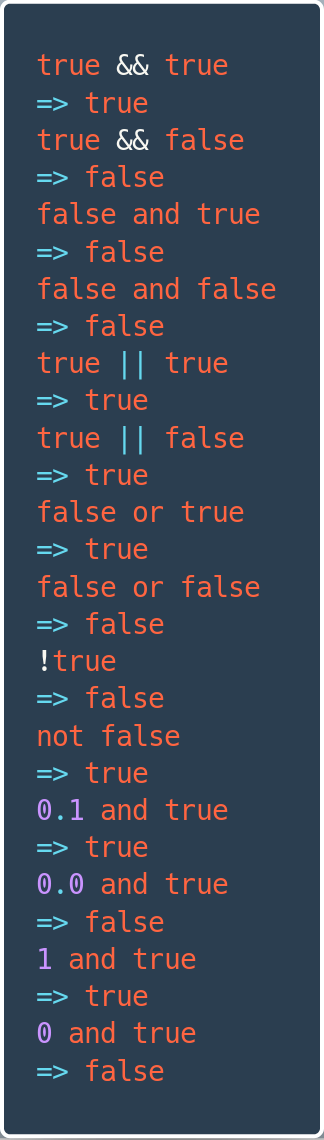
\includegraphics[width=0.20\textwidth]{logic.png}
    \caption{Logiska uttryck och hur de kan skrivas i CodEng.}
    \label{fig:logic1}
\end{figure}
\FloatBarrier

\subsection{Funktioner}
Funktioner i CodEng är kodstycken som har tilldelats variabelnamn. Funktionerna kan också bearbeta argument som skickats in i dem. Argumenten i funktioner till exempel vara någon av de datatyper som nämndes i under del 2.3. Funktioner kan anropas med ett funktionsanrop. Vid ett anrop utförs det kodstycke som tillhör just den funktionen på den plats i koden där anropet skrevs. I figur 4 visas en funktion skriven i textversionen av CodEng. När funktionen i figuren körs beräknas upphöjt till 3 för den siffra som skickades in till funktionen som argument och skriver ut svaret på beräkningen. Den gör sedan samma sak igen för de nio följande heltalen genom en \say{while-loop}. Det senaste uttrycket som kördes innan funktionen avslut är det värde som funktionen skickar ut. 

\FloatBarrier
\begin{figure}[h!]
    \centering
    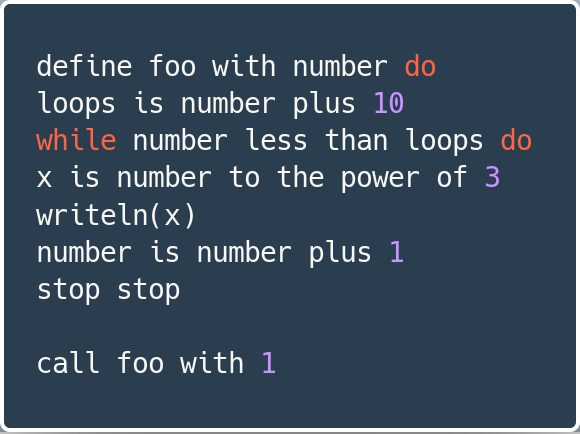
\includegraphics[width=0.35\textwidth]{function.png}
    \caption{En funktionsdeklaration och motsvarande anrop.}
    \label{fig:func1}
\end{figure}
\FloatBarrier


\subsection{Iterationer}
I CodEng finns endast en typ av iteration, \say{while}-loopar. \say{While}-loopen används för att köra ett kodstycke om och om igen tills oändligheten eller ett speciellt krav har uppfyllts. Själva loopen har sant respektive falskt läge. I det sanna läget körs kodstycket som står inne i loopen och i det falska läget stängs loopen av. I figur 5 visas ett exempel på en \say{while}-loop och hur de fungerar i språket. \say{While}-loopen körs på grund av att loop variabeln som satts till att vara \say{true} har placerats som loopens tillstånd. 

\FloatBarrier
\begin{figure}[h!]
    \centering
    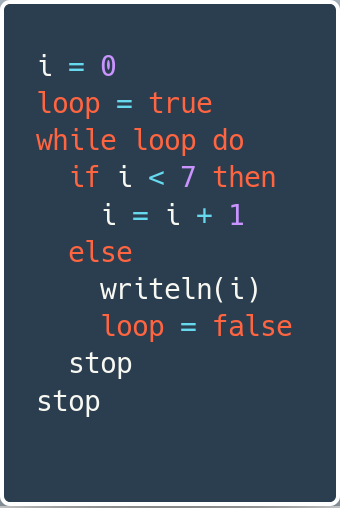
\includegraphics[width=0.35\textwidth]{while.png}
    \caption{En \say{while}-loop som visar på looping och val i loopar}
    \label{fig:while1}
\end{figure}
\FloatBarrier
\newpage
\subsection{Val}
De val som har implementerats i språket är de klassiska \say{if}- och \say{else}-satserna, översatt till svenska blir det om- och annars-satser. Satserna fungerar genom att koden inom just den \say{if}- eller \say{else}-satsen endast körs om det uttryck som tillhör satsen är sant. \say{If}-delen kollas först och om den delen är sann hoppas \say{else}-delen över, och tvärtom. Detta illustreras i samma figur 5, där uttrycket för \say{if}-delen är sann för siffrorna 0-6 men falsk när siffran blir 7. I detta läge körs istället koden för \say{else}-delen och loop-variabeln sätts till falsk, vilket gör att hela loopen stannar.

\subsection{Variabler och \say{Scope}}
\begin{wrapfigure}{r}{0.25\textwidth}
    \centering
    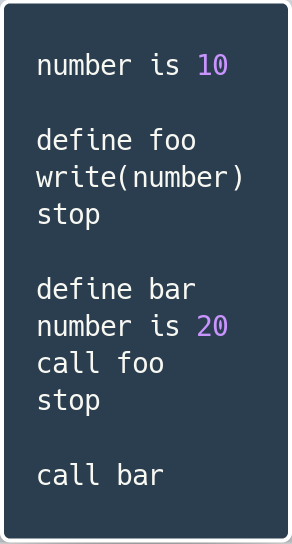
\includegraphics[width=0.25\textwidth]{scopecode.png}
    \caption{Exempel på hur \say{scope} fungerar i CodEng.}
\end{wrapfigure}
Variabler i CodEng består av bokstäver, siffror och understreck. Variabelnamn  kan inte bestå av endast siffror. Variablerna sparas med sitt värde i ett \say{scope}. CodEng har dynamiskt \say{scope}. Det innebär att variablens värde alltid är det första den hittar i sitt nuvarande scope. \\ \newline
Ett exempel på detta kan ses i figur 6 till höger. Figuren innehåller 3 \say{scopes}, ett som omsluter hela programmet och sedan har båda funktionerna varsitt \say{scope}. När foo kallas i bar kommer den att skriva ut \say{number}. Först letar foo i sitt eget scope efter \say{number} men hittar ingen deklarerad variabel med det namnet. Eftersom den kallades i funktionen bar letar den nu i dess scope och hittar att den har värdet 20. Om det hade varit statiskt \say{scope} istället för dynamiskt så kommer foo att leta efter variabeln i \say{scopet} för hela programmet istället, då det är där funktionen är definerad, och värdet blir då 10.
\newpage
\section{Systemdokumentation}
\subsection{Systembeskrivning}
CodEng är skrivet med hjälp av en redan skriven parser kallad rdparse. Parsern gör först en lexikalisk analys för att konstruera tokens. Därefter parsas alla token och matchar mot skrivna regler för att skapa ett program. Programmet skapas enligt en trädstruktur av noder, det vill säga blir programmet ett stort \say{constraint-network}.
\subsection{Lexikalisk analys}
I CodEngs lexer skapas tokens med hjälp av reguljära uttryck. Dessa tokens är sorterade i prioriteringsordning och grupperade efter typ. 
Först tas alla \say{whitespaces} och kommentarer bort ur koden då de inte används. Sedan skapas tokens och objekt i följande ordning:
\begin{itemize}
\item Strings - CEString-objekt skapas med innehållet mellan två citattecken.
\item Bool - CEBool-objekt skapas med nyckelorden true eller false.
\item Numbers - CEFloat-objekt skapas av decimaltal och CEInteger-objekt skapas med heltal.
\item Keywords - Matchar alla nyckelord som används och skapar tokens.
\item Operators - Matchar alla operatorer och skapar tokens. ex. ==, +, ** eller equal to, plus, to the power of.
\item Variables - CEVariable-objekt skapas av resterande ord som följer regex-matchningen.
\end{itemize}
Ifall det finns tecken kvar som inte matchade till något skickas ett felmeddelande ut till användaren.
\subsection{Parsning}
Parsern använder sig av språkets grammatiska definition för att matcha tokens till korrekt skrivna uttryck. Dessa regler är specificerade under avsnitt 3.5. \newline Parsern är strukturerad så att vid korrekta uttryck skapas noder. Noderna är interna för språket och användaren kan inte komma åt dem. De binder ihop flera objekt eller noder i ett träd. Vid körning så används \say{assess}-metoden på programnoden som i sin tur går igenom trädet för att köra programmet. I exemplet nedan sker en variabeltilldelning, en räkneoperation och en utskrift av en siffra.
\newpage
\newline \center\textbf{\textttf{x = 4 + 6}}
\center \textbf{\textttf{write(12)}}

\begin{figure}[h!]
    \centering
    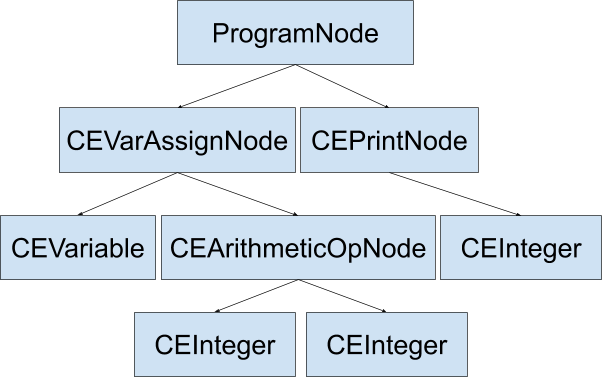
\includegraphics[width=0.60\textwidth]{nodeuml.png}
    \caption{Ett nodträd}
\end{figure}

\subsection{Noder och \say{assess}}
\begin{flushleft}
Alla noder har en gemensam metod: \say{assess}. När \say{assess} kallas på en nod eller ett objekt utvärderar det sitt värde och returnerar det. Ifall värdet beror på andra objekt kallas metoden på de objekten först. Metoden tar in scope som enda argument. Ifall noden har ett eget kodblock skapas ett nytt scope som sedan skickas med som argument när noden kör \say{assess} på blocket. Datatyperna returnerar sig själva när assess kallas på dem. 
\end{flushleft}
\newpage
\subsection{Grammatik(BNF)}
\begin{alltt}
<PROGRAM>           ::= <BLOCK>

<BLOCK>             ::= <BLOCK> <STATEMENT>
                    |   <STATEMENT>

<STATEMENT>         ::= <IF_STATEMENT>
                    |   <FUNC_DEF>
                    |   <FUNC_CALL>
                    |   <WHILE_LOOP>
                    |   <PRINT_STATEMENT>
                    |   <VALID>

<IF_STATEMENT>      ::= "if" <EXPR> "then" <BLOCK> "else" <BLOCK> "stop"
                    |   "if" <EXPR> "then" <BLOCK> "else" <BLOCK> "end"
                    |   "if" <EXPR> "then" <BLOCK> "stop"
                    |   "if" <EXPR> "then" <BLOCK> "end"
                        
<FUNC_DEF>          ::= "define" <CEVARIABLE> "with" <ARG_LIST> <BLOCK> "stop"
                    |   "define" <CEVARIABLE> "with" <ARG_LIST> <BLOCK> "end"
                    |   "define" <CEVARIABLE> <BLOCK> "stop"
                    |   "define" <CEVARIABLE> <BLOCK> "end"

<FUNC_CALL>         ::= "call" <VAR> "with" <ARG_LIST>
                    |   "call" <VAR>
                    
<ARG_LIST>          ::= <ARG_LIST> "," <ARG_DECL>
                    |   <ARG_DECL>
                    
<WHILE_LOOP>        ::= "while" <EXPR> "do" <BLOCK> "stop"
                    |   "while" <EXPR> "do" <BLOCK> "end"
                    
<PRINT_STATEMENT>   ::= "write" "(" <ARG_LIST> ")"
                    |   "writeln" "(" <ARG_LIST> ")"            
                    
<VALID>             ::= <ASSIGN>
                    |   <EXPR>
                    
<ASSIGN>            ::= <VAR> "=" <EXPR>
                    |   <VAR> "is" <EXPR>
                    
<EXPR>              ::= <LOGIC_OR>

<LOGIC_OR>          ::= <LOGIC_OR> "||" <LOGIC_AND>
                    |   <LOGIC_OR> "or" <LOGIC_AND>
                    
<LOGIC_AND>         ::= <LOGIC_OR> "&&" <COMPARE_EQUALITY>
                    |   <LOGIC_OR> "and" <COMPARE_EQUALITY>
                    
<COMPARE_EQUALITY>  ::= <COMPARE_EQUALITY> "==" <COMPARE_RELOPS>
                    |   <COMPARE_EQUALITY> "equal to" <COMPARE_RELOPS>
                    |   <COMPARE_EQUALITY> "!=" <COMPARE_RELOPS>
                    |   <COMPARE_EQUALITY> "not equal to" <COMPARE_RELOPS>
                    |   <COMPARE_RELOPS>
                    
<COMPARE_RELOPS>    ::= <COMPARE_RELOPS> "<" <ARITHMETIC_EXPR>
                    |   <COMPARE_RELOPS> "less than" <ARITHMETIC_EXPR>
                    |   <COMPARE_RELOPS> "<=" <ARITHMETIC_EXPR>
                    |   <COMPARE_RELOPS> "less than or equal to" <ARITHMETIC_EXPR>
                    |   <COMPARE_RELOPS> ">" <ARITHMETIC_EXPR>
                    |   <COMPARE_RELOPS> "greater than" <ARITHMETIC_EXPR>
                    |   <COMPARE_RELOPS> "=>" <ARITHMETIC_EXPR>
                    |   <COMPARE_RELOPS> "greater than or equal to" <ARITHMETIC_EXPR>
                    |   <ARITHMETIC_EXPR>
                    
<ARITHMETIC_EXPR>   ::= <ARITHMETIC_EXPR> "+" <TERM>
                    |   <ARITHMETIC_EXPR> "plus" <TERM>
                    |   "add" <ARITHMETIC_EXPR> "to" <TERM>
                    |   <ARITHMETIC_EXPR> "-" <TERM>
                    |   <ARITHMETIC_EXPR> "minus" <TERM>
                    |   "subtract" <ARITHMETIC_EXPR> "from" <TERM>
                    |   <TERM>
                    
<TERM>              ::= <TERM> "*" <FACTOR>
                    |   <TERM> "times" <FACTOR>
                    |   "multiply" <TERM> "by" <FACTOR>
                    |   <TERM> "/" <FACTOR>
                    |   <TERM> "over" <FACTOR>
                    |   "divide" <TERM> "by" <FACTOR>
                    |   <FACTOR>
                    
<FACTOR>            ::= <EXP> "**" <FACTOR> 
                    |   <EXP> "to the power of" <FACTOR>
                    |   "!" <EXP>
                    |   "not" <EXP>
                    |   <EXP>
\newpage         
<EXP>               ::= "(" <EXPR> ")"
                    |   <BOOL_CONST>
                    |   <NUM>
                    |   <STRING>
                    |   <VAR>

<BOOL_CONST>        ::= "true"
                    |   "false"
                    
<NUM>               ::= <CEINTEGER>
                    |   <CEFLOAT>
                    
<STRING>            ::= <CESTRING>

<VAR>               ::= <CEVARIABLE>
\end{alltt}

\newpage
\section{Erfarenheter och reflektion}
\begin{flushleft}
Under projektets gång känner vi att vi fått mycket mer ingående kunskaper angående hur ett programmeringsspråk är uppbyggt från grammatikregler till tokenuppbyggnad via lexern och parserns roll i hur programmeringsspråk körs som trädstrukturer.
\\ \newline
Jämför vi mot de tidigare idéer som vi hade syns det att grundidén med att kunna skriva ut språket som text finns kvar och är implementerad i minst ett fall för allt utom parenteser och siffror. Dock ser koden inte ut som \say{vanlig} text som det var tänkt från början och många synonymer implementerades inte. Språket kan utökas med synonymer väldigt enkelt genom att lägga till ett token i lexern. Hade vi känt att vi hade haft nog med tid skulle det varit roligt att ha försökt implementerat en funktion/metod som gjorde om textskrivna tal till våra egna datatyper för Floats och Integers. Eftersom vi underskattade svårigheterna som uppstod under implementationsarbetets gång skalade vi tillbaka språket kontinuerligt. Språket är inte objektsorienterat för det går inte att genom CodEng kod initiera nya klasser. \\ \newline
Den del som tog mest tid under implementationen var att skriva koden för hur scopes skulle fungera och interagera med alla andra delar som vi tidigare hade implementerat. Om ett liknande projekt görs i framtiden där ett programmeringsspråk skulle skrivas är scope den del som borde implementeras först då alla andra delar av språket är på något sätt beroende på hur det fungerar. \\ \newline
Programmeringsspråket Ruby var riktigt roligt och intuitivt att lära sig och använda sig av i den här projektkursen. I efterhand borde vi nog studerat rdparse.rb mer innan vi började på projektets implementationsdel, för att undvika att skriva om kodstycken som inte är kompatibla med parsern.
\end{flushleft}
\end{document}
